% Diapo d'intro
\begin{frame}[c]
  \frametitle{Context}
%rajouter le titre (version courte) dans toute les slides
\begin{center}
  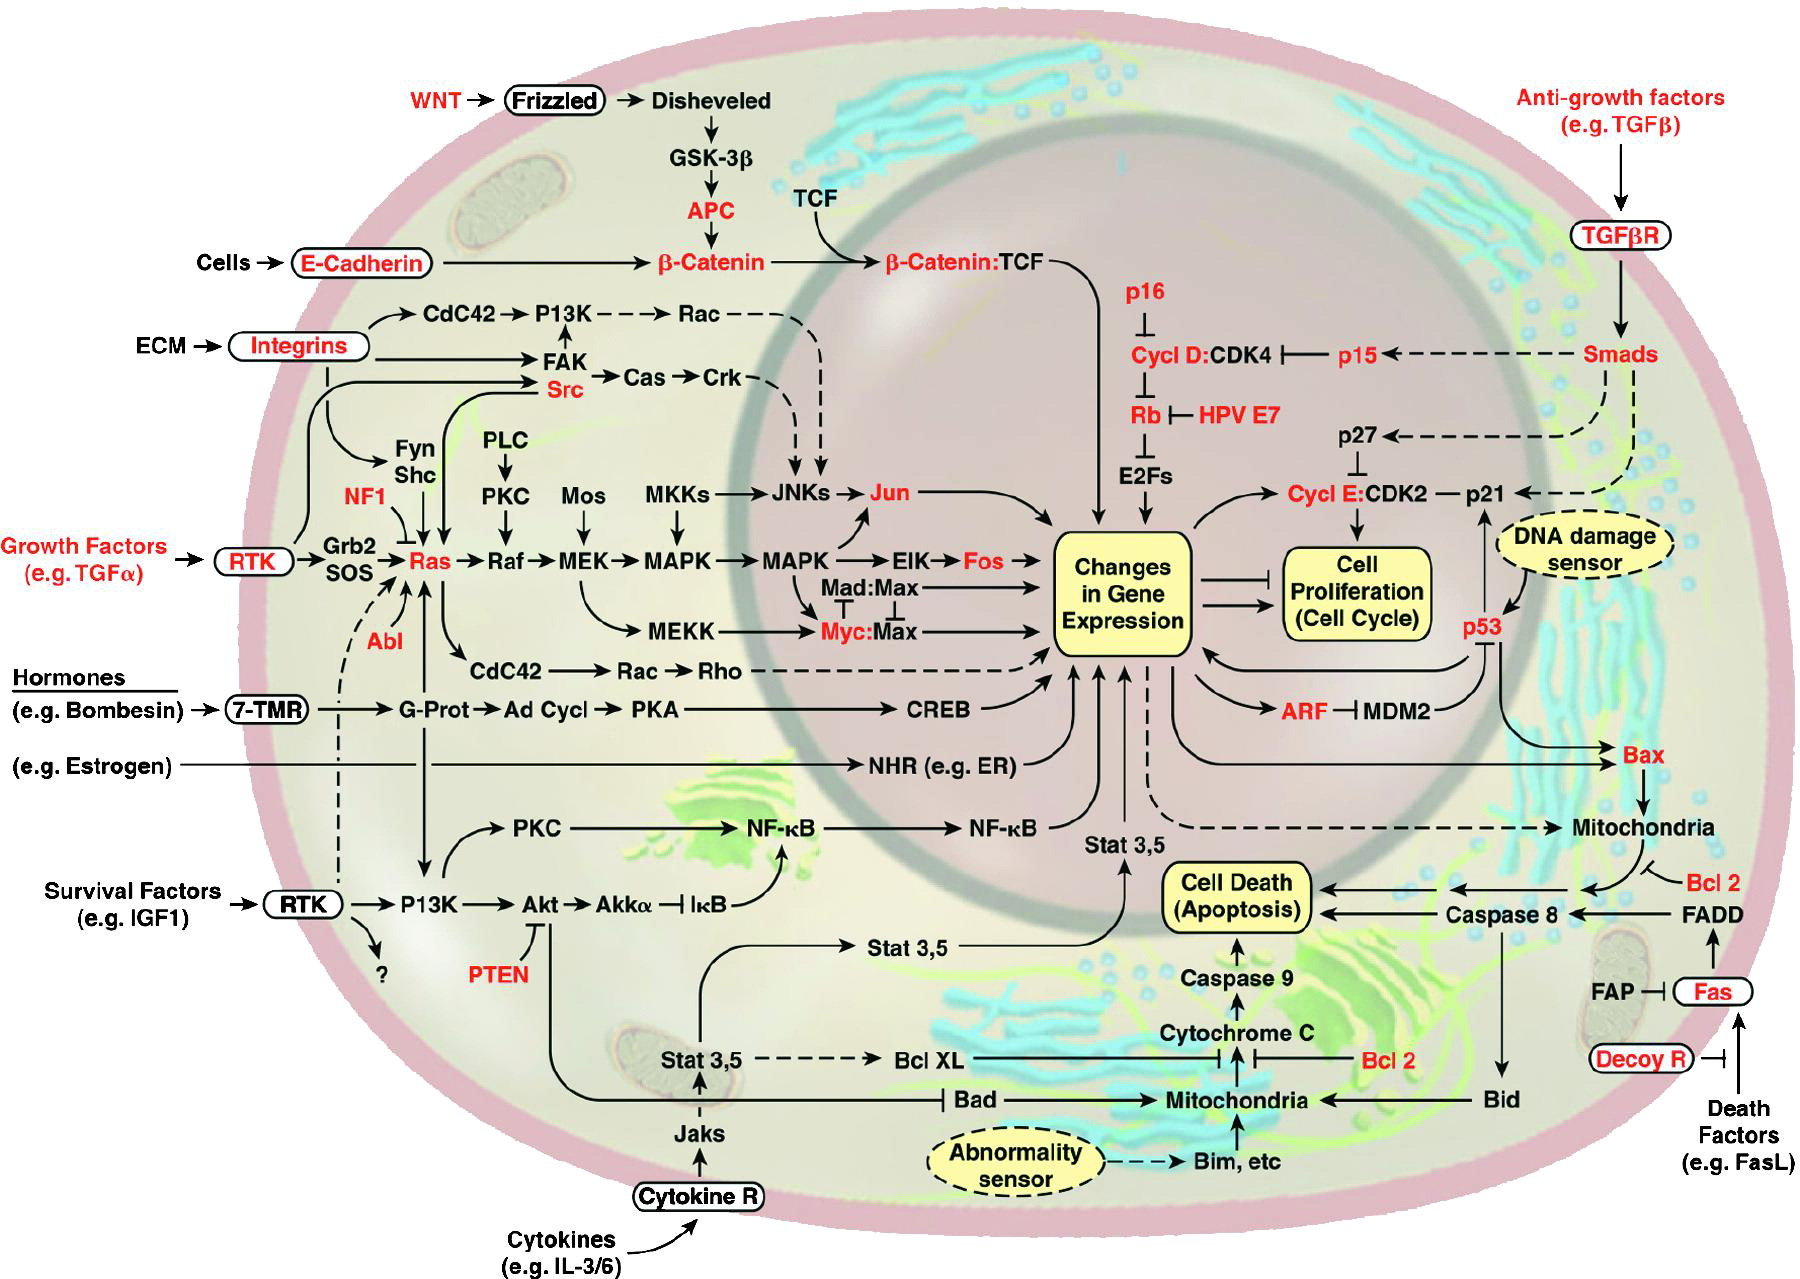
\includegraphics[scale=0.12]{images/cellule-description.jpeg}
\end{center}
\begin{center}
{\tiny \color{darkgreen}[\citelui]}
\end{center}

%\tcite{Wikipédia}

\begin{itemize}
\item Cellular processes are driven by networks of biological interactions.
\item Formal modelling and analysis of Biological Regulatory Network.
\item Static analysis of qualitative and quantitative properties.
\end{itemize}

%Cellular processes are driven by networks of biological reactions. Cells rely on the tight coordination of these pathways to achieve proper functioning.
%With the help of signaling pathway, a cell senses changes in its environnement or internal state. This information is then passed on via cascades of biochemical 
%reactions to the appropriate mechanisms which respond by modifying the metabolic and transcriptiona activities. this in turn modifies the behavior of the cell.

%Consequently, the dynamics of biopathways play a crucial role in determinig cellular functions.

%Examples: circadian rhythm, the apoptosis pathway inducing programmed cell death, cell differentiation.

%\textcolor{couleurtheme}{$\Rightarrow$} \fbox{\tval{\large The need of comprehension of biological systems}} \textcolor{couleurtheme}{$\Leftarrow$}


%\textcolor{couleurtheme}{$\Rightarrow$} \fbox{\tval{\large Allow efficient translation from Process Hitting to BRN}} \textcolor{couleurtheme}{$\Leftarrow$}

\end{frame}


